\documentclass{article}
\usepackage{graphicx}
\usepackage{imakeidx}
\makeindex
\usepackage[utf8]{inputenc}
\usepackage[document]{ragged2e}
\usepackage{graphicx}

\renewcommand{\contentsname}{Indice}
\begin{document}
	\begin{centering}
    \vspace*{0.5 cm}
    \textsc{\LARGE Universidade do Minho}\\[2.0 cm]	% University Name
	\textsc{\LARGE Engenharia Informática}\\[1 cm]				% Course Code
	\textsc{\large 21/22}\\[0.5 cm]				% Course Name
	\rule{\linewidth}{0.2 mm} \\[0.4 cm]
	{ \huge \bfseries Redes - TP2}
	\rule{\linewidth}{0.2 mm} \\[1.5 cm]
		\begin{minipage}{0.4\textwidth}
		\begin{flushright}\large
		\begin{raggedright}
		Afonso Amorim A97569\par
		Luís Ferreira A95111\par
		Pedro Dantas  A97396\par
		\end{raggedright}
		\end{flushright}
	\end{minipage}
	\end{centering}
\clearpage
\tableofcontents
\cleardoublepage
\section{Parte 1}
\subsection{Exercício 1}
1. Prepare uma topologia CORE para verificar o comportamento do
traceroute. Na topologia deve existir: um host (pc) cliente designado Bela cujo router de acesso é R2; o router R2 está simultaneamente ligado a dois routers R3 e R4; estes estão conectados a um router R5, que por sua vez, se liga a um host (servidor) designado Monstro. Ajuste o nome dos equipamentos atribuídos por defeito para o enunciado. Nas ligações ( links) da rede de core estabeleça um tempo de propagação de 10ms. Após ativar a topologia, note que pode não existir conectividade IP imediata entre a Bela e o Monstro até que o anúncio de rotas entre routers estabilize.

\begin{center}
\includegraphics[width=12cm, height= 4 cm]{Images/EsquemaEx1.png}
\caption{\textit{Fig. 1 - Modelo topologia CORE}}
\vspace{1.5 cm}
\end{center}


\subsubsection{Alínea a)}
\textbf{Active o \textit{wireshark} ou o \textit{tcpdump} no host \textit{Bela}. Numa shell de \textit{Bela} execute o comando \textit{traceroute -I} para o endereço IP do \textit{Monstro}}\par
\vspace{1 cm}
\begin{center}
    \includegraphics[width=12cm]{Images/Ex1a.png}
\caption{\textit{Fig. 2 - Execução do comando \textit{traceroute}}}
\vspace{2 cm}
\end{center}


\subsubsection{Alínea b)}
\textbf{Registe e analise o tráfego ICMP enviado pelo sistema Bela e o tráfego ICMP recebido como resposta. Comente os resultados face ao comportamento esperado.}\par
\vspace{0.5 cm}
\begin{center}
    \includegraphics[width=12cm]{Images/Ex1b.png}
\caption{\textit{Fig. 3 - Pacotes Recebidos}}
\par\vspace{0.5cm}
\end{center}

\hspace{0.5cm}Como podemos ver, os pacotes são enviados em conjuntos de 3. Podemos também observar que os primeiros 3 conjuntos (TTL $<$ 4) não conseguem chegar ao destino, pelo que devolvem uma mensagem de erro. \par\vspace{0.35cm}

\subsubsection{Alínea c)}
\textbf{Qual deve ser o valor inicial mínimo do campo TTL para alcançar o servidor Monstro ? Verifique na prática que a sua resposta está correta.}\par
\vspace{0.35 cm}
\begin{center}
    \includegraphics[width= 12 cm]{Images/Ex1c.png}
\caption{\textit{Fig. 4 - TTL Mínimo}}\par\vspace{0.02cm}
\end{center}

\hspace{0.5cm}Como pudemos verificar no exercício anterior, é necessário um TTL mínimo igual a 4.\par\clearpage

\subsubsection{Alínea d)}
\textbf{Calcule o valor médio do tempo de ida-e-volta (RTT - Round-Trip Time) obtido no acesso ao servidor. Para melhorar a média, poderá alterar o número pacotes de prova com a opção -q.}\par
\begin{center}
\includegraphics[width = 12 cm]{Images/Ex1d.png}\par
\caption{\textit{Fig. 5 - Tempo de ida-e-volta}}\par\vspace{0.35cm}
\end{center}


\hspace{0.5cm}Como podemos verificar na Figura 5, enviamos 10 pacotes e recebemos o tempo que demoram a ir e voltar. Para calcular o tempo médiio de ida-e-volta utilizamos os valores na \textit{linha 4} e fazemos a média de todos eles.\par
\vspace{0.5}
\textit{\small(82.740+82.731+81.917+81.873+81.917+81.873+82.018+81.965+81.952+81.943+82.562+82.509)/10}\par
Ficamos assim a saber que o tempo médio de ida-e-volta é de 82.221 ms.\vspace{0.35cm}

\subsubsection{Alínea e)}
\textbf{O valor médio do atraso num sentido ( \textit{One-Way Delay}) poderia ser calculado com precisão dividindo o RTT por dois? O que torna difícil o cálculo desta métrica?}\par
\vspace{0.35 cm}
\hspace{0.5cm}Não, o valor não pode ser calculado dividindo o RTT por dois porque ao fazer isso estaríamos a assumir que o tempo de ida e volta eram exatamente iguais, o que pode não acontecer. Ao voltar o pacote pode tomar um caminho diferente do caminho de ida e demorar mais ou menos tempo.
\cleardoublepage
\subsection{Exercício 2}


\begin{center}
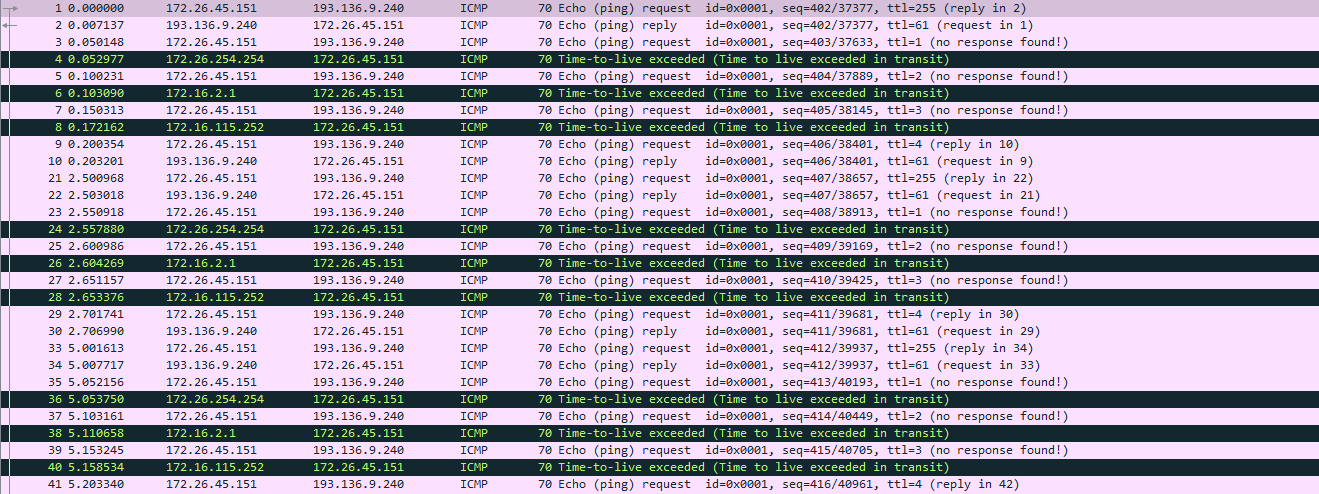
\includegraphics[width=13cm]{unknown.png}\par\caption{\textit{Fig. 6 - Tráfego ICMP}}\par
\end{center}

\subsubsection{Alínea a)}\par\vspace{0.5cm}
\begin{center}

\includegraphics[width=12cm]{ip.png}\par\caption{\textit{Fig. 7 - IP}}\par\vspace{0.3cm}
\end{center}

\textbf{Qual é o endereço IP da interface ativa do seu computador?}\par\vspace{0.35cm}
\hspace{0.5cm}Como é possível observar na figura 7, o endereço IP da interface ativa do nosso computador é: \textbf{172.26.45.151}\par\vspace{0.35cm}

\subsubsection{Alínea b)}\par\vspace{0.5cm}
\begin{center}
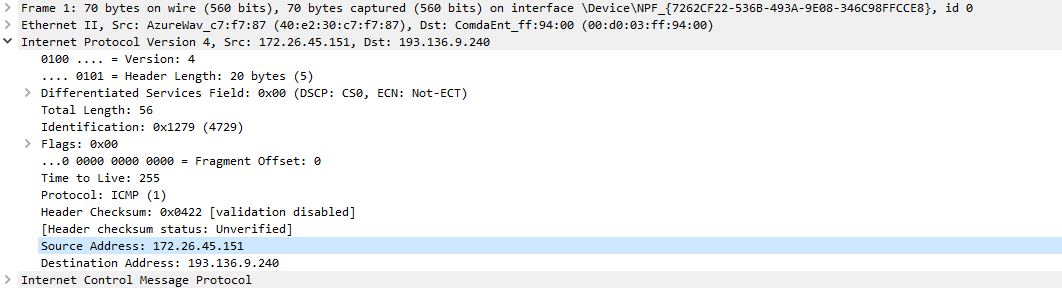
\includegraphics[width=12cm]{wda.png}\par\caption{\textit{Fig. 8 - Valores dos campos de um Pacote}}\par\vspace{0.5cm}
\end{center}

\textbf{Qual é o valor do campo protocolo? O que permite identificar?}\par\vspace{0.35cm}
\hspace{0.5cm}Como podemos verificar na figura 8, o valor do campo protocolo é \textbf{1}, sendo que este identifica o protocolo \textbf{ICMP} (\emph{Internet Control Message Protocol}).

\subsubsection{Alínea c)}

\textbf{Quantos \emph{bytes} tem o cabeçalho IPv4? Quantos \emph{bytes} tem o campo de dados (\emph{payload}) do datagrama? Como se calcula o tamanho do \emph{payload}?}\par\vspace{0.35cm}
\hspace{0.5cm}Através da análise da figura 8, podemos conferir que o cabeçalho IP(v4) possui um tamanho de 20 \emph{bytes}. Tendo em conta que o campo do datagrama pode ser obtido através da diferença entre o tamanho do pacote (56 \emph{bytes}) e o tamanho do cabeçalho, concluímos que este tem um tamanho de 36 \emph{bytes}.\vspace{0.25cm}

\subsubsection{Alínea d)}

\textbf{O datagrama IP foi fragmentado? Justifique.}\par\vspace{0.35cm}
\hspace{0.5cm}Tendo em conta novamente a figura 8, podemos verificar que o pacote não foi fragmentado. Isto porque tanto o valor da \emph{flag} como o do \emph{fragment offset} estão a 0.\vspace{0.35cm}

\subsubsection{Alínea e)}\vspace{0.1cm}

\begin{center}
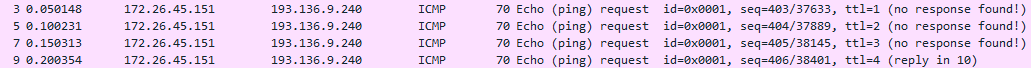
\includegraphics[width=12cm]{2.png}\par\caption{\textit{Fig.9 - Série de Pacotes Ordenados pelo Endereço Fonte}}\par\vspace{0.1cm}
\end{center}
\begin{center}
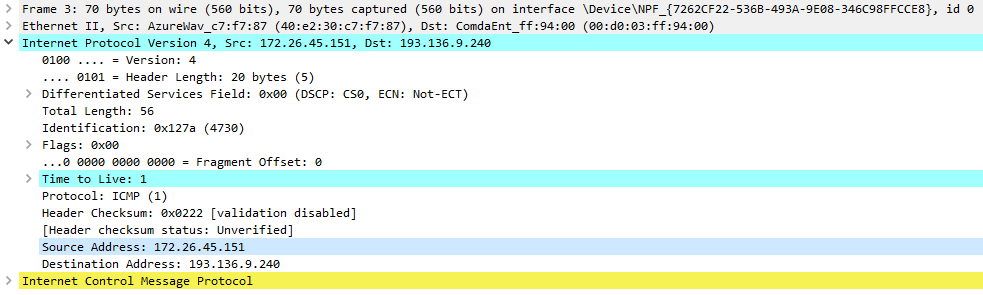
\includegraphics[width=12cm]{3.png}\par\caption{\textit{Fig. 10 - Pacote 1}}\par\vspace{0.2cm}
\end{center}
\begin{center}
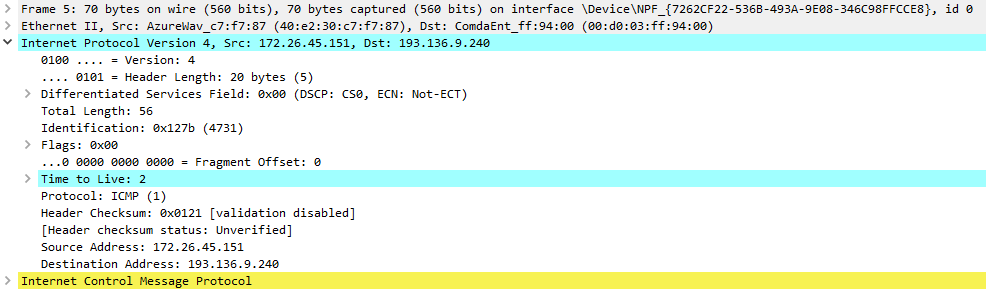
\includegraphics[width=12cm]{4.png}\par\caption{\textit{Fig. 11 - Pacote 2}}\par\vspace{0.3cm}
\end{center}
\begin{center}
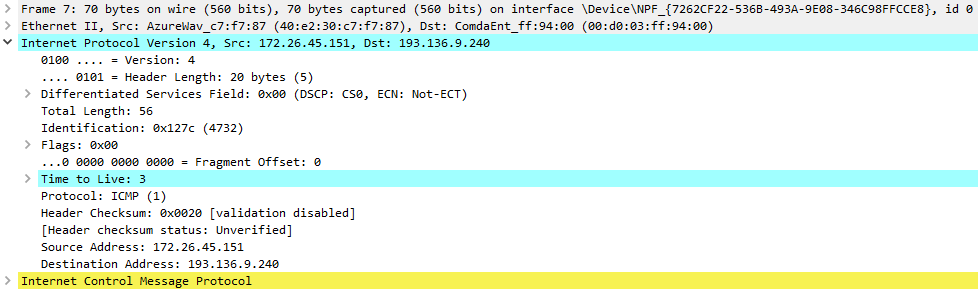
\includegraphics[width=12cm]{5.png}\par\caption{\textit{Fig. 12 - Pacote 3}}\par\vspace{0.5cm}
\end{center}
\begin{center}
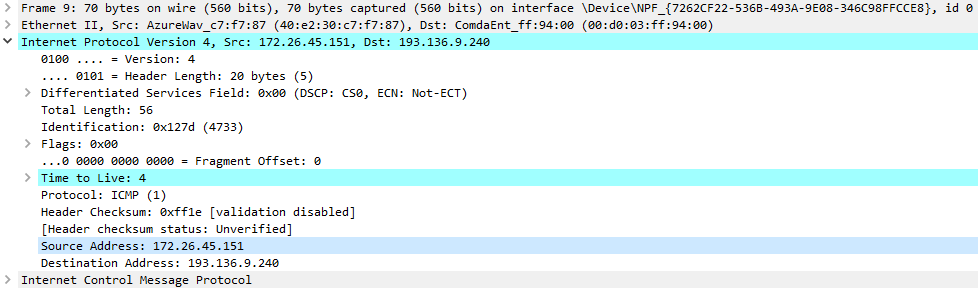
\includegraphics[width=12cm]{6.png}\par\caption{\textit{Fig. 13 - Pacote 4}}\par\vspace{0.5cm}
\end{center}

\textbf{Ordene os pacotes capturados de acordo com o endereço IP fonte (e.g., selecionando o cabeçalho da coluna
\emph{Source}), e analise a sequência de tráfego ICMP gerado a partir do endereço IP atribuído à interface da sua
máquina. Para a sequência de mensagens ICMP enviadas pelo seu computador, indique que campos do cabeçalho IP variam de pacote para pacote.}\par\vspace{0.35cm}
\hspace{0.5cm}Como podemos observar nas figuras 10, 11, 12 e 13, os campos do cabeçalho IP que variam de pacote para pacote são o \emph{\textbf{TTL}} e o \emph{\textbf{Identification}}.\vspace{0.35cm}

\subsubsection{Alínea f)}\par

\textbf{Observa algum padrão nos valores do campo de Identificação do datagrama IP e TTL?}\par\vspace{0.35cm}
\hspace{0.5cm}Analisando as figuras anteriormente referidas podemos verificar que, de facto, existe um padrão nos campos referidos, sendo que ambos têm um incremento de \textbf{1} de pacote em pacote.\vspace{0.3cm}

\subsubsection{Alínea g)}\par\vspace{0.5cm}
\begin{center}
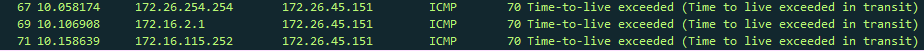
\includegraphics[width=12cm]{7.png}\par\caption{\textit{Fig.14 - Série de Pacotes Ordenados Pelo Endereço Destino}}\par\vspace{0.5cm}
\end{center}
\begin{center}
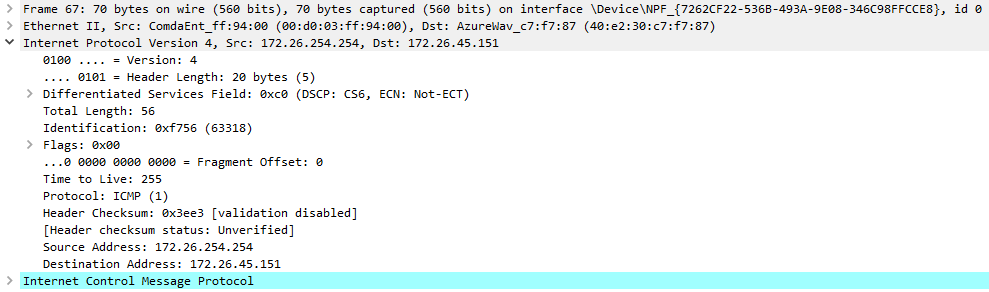
\includegraphics[width=12cm]{8.png}\par\caption{\textit{Fig. 15 - Pacote 1}}\par\vspace{0.5cm}
\end{center}
\begin{center}
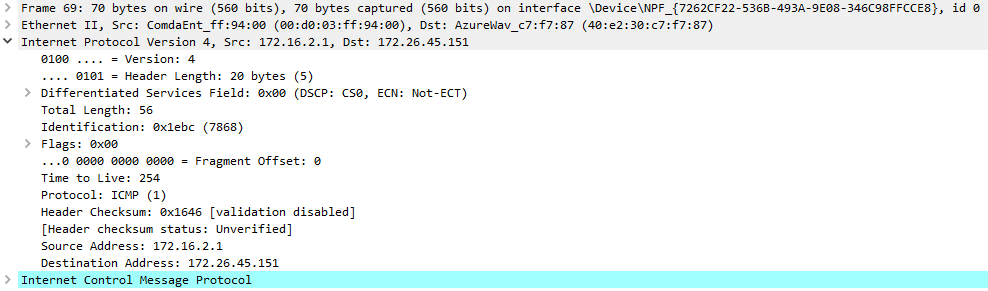
\includegraphics[width=12cm]{9.png}\par\caption{\textit{Fig.16 - Pacote 2}}\par\vspace{0.5cm}
\end{center}
\begin{center}
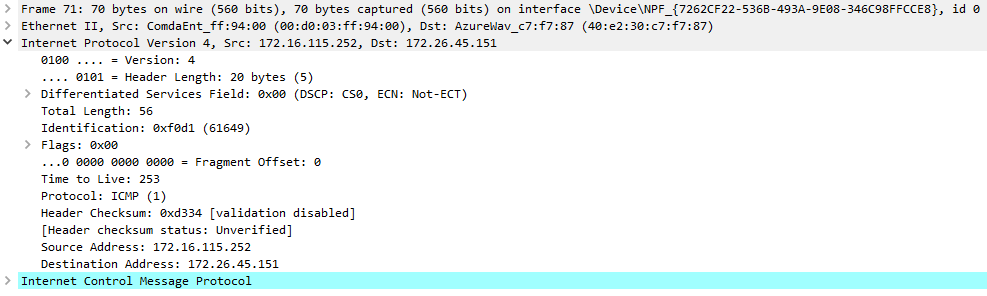
\includegraphics[width=12cm]{10.png}\par\caption{Fig. 17 - \textit{Pacote 3}}\par\vspace{2cm}
\end{center}

\textbf{Ordene o tráfego capturado por endereço destino e encontre a série de respostas ICMP TTL \emph{exceeded} enviadas
ao seu computador. Qual é o valor do campo TTL? Esse valor permanece constante para todas as mensagens de
resposta ICMP TTL \emph{exceeded} enviados ao seu \emph{host}? Porquê?}\par\vspace{0.35cm}
\hspace{0.5cm}As figuras 15, 16 e 17 mostram, entre outros campos, os valores \emph{\textbf{TTL}} dos respectivos pacotes. Assim, podemos observar que o primeiro pacote tem \textbf{\emph{TTL} = 255}, o segundo \textbf{\emph{TTL} = 254} e o terceiro \textbf{\emph{TTL} = 253}. A diminuição neste campo deve-se ao facto de que, quando é necessário o envio de uma mensagem de erro, os pacotes são enviados de \emph{routers} mais distantes, fazendo com que, no caminho de regresso, estes passem por mais \emph{routers} intermédios, contribuindo então para o decremento referido.\par\clearpage

\begin{center}
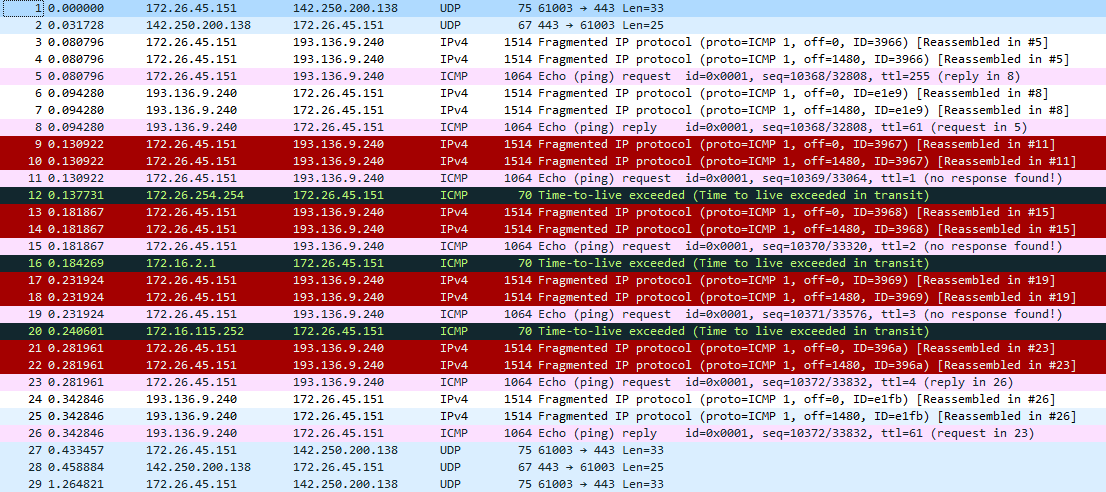
\includegraphics[width=13cm]{awwd.png}\par\caption{\textit{Fig. 18 - Pacotes com Fragmentação}}
\end{center}
\subsection{Exercício 3}

\subsubsection{Alínea a)}
\begin{center}
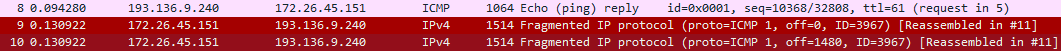
\includegraphics[width=14cm]{pacote.png}\par\caption{\textit{Fig. 19 - Pacote 1 e Fragmentação}}\par\vspace{0.3cm}
\end{center}

\textbf{Localize a primeira mensagem ICMP. Porque é que houve necessidade de fragmentar o pacote inicial?}\par\vspace{0.35cm}
\hspace{0.5cm}Tendo em conta que a \textbf{MTU} (\emph{Maximum Transmission Unit}) que foi utilizada tinha capacidade para enviar pacotes com um tamanho máximo de apenas 1500 \emph{bytes} e o nosso pacote possuía um tamanho de 4010 \emph{bytes}, houve necessidade deste mesmo pacote ser fragmentado de forma que possibilitasse o seu envio.\par\vspace{0.35cm}


\subsubsection{Alínea b)}
\begin{center}
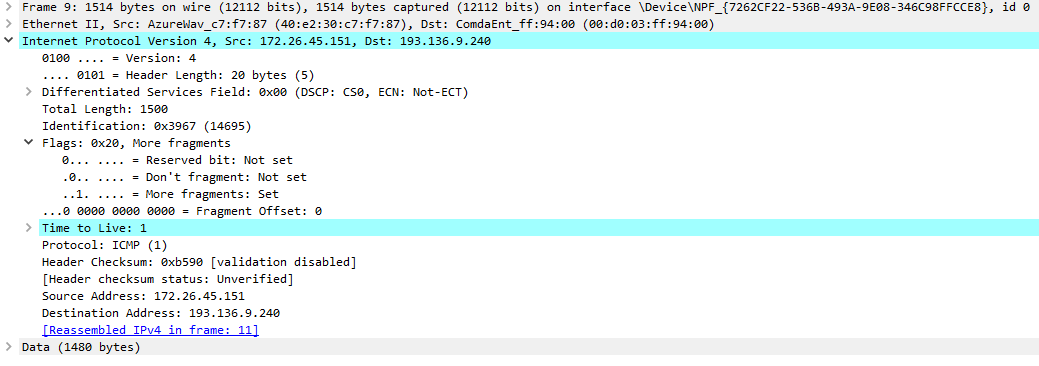
\includegraphics[width=12cm]{hr.png}\par\caption{\textit{Fig. 20 - Fragmento 1 do Pacote 1}}\par\vspace{0.3cm}
\end{center}

\textbf{Imprima o primeiro fragmento do datagrama IP segmentado. Que informação no cabeçalho indica que o
datagrama foi fragmentado? Que informação no cabeçalho IP indica que se trata do primeiro fragmento? Qual é o tamanho deste datagrama IP?}\par\vspace{0.35cm}
\hspace{0.5cm}O campo que nos permite averiguar se um pacote foi ou não fragmentado são as \emph{flags}. Podemos identificar o primeiro fragmento através dos valores do \emph{fragment offset} (que deve ter o valor \textbf{0}) e do \emph{more fragments} (que deve ter o valor \textbf{1}, indicando a existência de mais fragmentos). Desta forma, e como podemos observar na figura 20, esta representa o primeiro fragmento. O tamanho deste datagrama IP é de 1500 \emph{bytes}.\par\clearpage

\subsubsection{Alínea c)}
\begin{center}
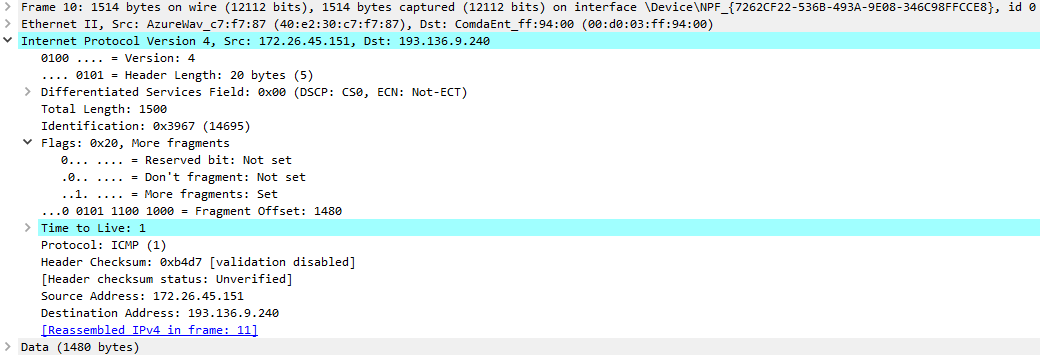
\includegraphics[width=12cm]{1243.png}\par\caption{\textit{Fig. 21 - Fragmento 2 do Pacote 1}}\par\vspace{0.3cm}
\end{center}
\textbf{Imprima o segundo fragmento do datagrama IP original. Que informação do cabeçalho IP indica que não se trata do 1º fragmento? Há mais fragmentos? O que nos permite afirmar isso?}\par\vspace{0.35cm}
\hspace{0.5cm}O campo que nos indica que não se trata do 1º fragmento é, como foi explicado anteriormente, o \emph{fragment offset} que, como podemos ver na figura 21, é diferente de \textbf{0}. Podemos também verificar o facto de que existem mais fragmentos, visto que o valor do \emph{more fragments} é \textbf{1}.\vspace{0.35cm}

\subsubsection{Alínea d)}
\begin{center}
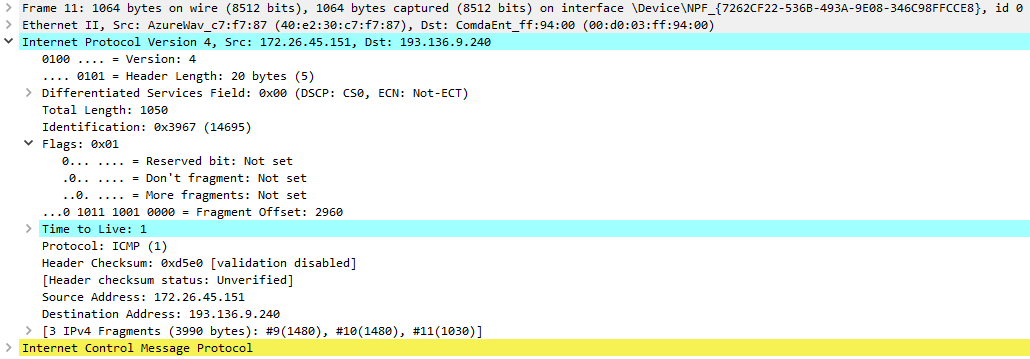
\includegraphics[width=12cm]{awfa.png}\par\caption{\textit{Fig. 22 - Fragmento 3 do Pacote 1}}\par\vspace{0.3cm}
\end{center}

\textbf{Quantos fragmentos foram criados a partir do datagrama original? }\par\vspace{0.35cm}
\hspace{0.5cm}Podemos verificar se um fragmento é o último, mais uma vez, através das \emph{flags}. Neste caso, o último fragmento terá um valor de \textbf{0} na \emph{flag} \emph{more fragments} e um valor diferente de \textbf{0} na \emph{fragment offset}. Isto verifica-se na figura 22, pelo que podemos concluir que o número total de fragmentos criados é \textbf{3}.\par\vspace{0.35cm}

\subsubsection{Alínea e)}
\textbf{Indique, resumindo, os campos que mudam no cabeçalho IP entre os diferentes fragmentos, e explique a forma como essa informação permite reconstruir o datagrama original.}

\vspace{0.35cm}

\hspace{0.5cm}Os campos nos quais se verificam alterações nos diferentes fragmentos são, como referido anteriormente, as \emph{flags}, nomeadamente o \emph{fragment offset} e o \emph{more fragments}. Estes têm as funções de nos indicar a ordem pela qual os fragmentos devem ser organizados e se existem ou não mais fragmentos, respetivamente. A ordem pela qual se organizam é especialmente importante para a reconstrução do datagrama original, tendo em conta que isto será possível se os fragmentos forem organizados por ordem crescente.\par\vspace{0.35cm}

\subsubsection{Alínea f)}
\textbf{Verifique o processo de fragmentação através de um processo de cálculo.}\par\vspace{0.35cm}

\hspace{0.5cm}Como referido anteriormente, o pacote original foi dividido em três fragmentos, sendo que dois deles têm um tamanho de 1500 \textit{bytes} e um deles tem tamanho de 1010 \textit{bytes}. No entanto, devemos retirar os valores dos cabeçalhos a dois destes fragmentos, de modo a obter o tamanho real do pacote original. Desta forma, aos 4010\textit{ bytes} retiramos 40 \textit{bytes} pertencentes aos cabeçalhos, sobrando então os \textbf{3070 \textit{bytes}} que representam, de facto, o tamanho do pacote original. (1480 + 1480 + 1010 + 40 = 4010)\par\vspace{0.35cm}


\subsubsection{Alínea g)}
\textbf{Escreva uma expressão lógica que permita detetar o último fragmento correspondente ao datagrama original.}\par\vspace{0.35cm}
\hspace{0.5cm} De modo a possibilitar a deteção do último fragmento do datagrama original, devemos ter em atenção as duas \textit{flags} referidas em perguntas anteriores: \textit{more fragments} e \textit{fragment offset}. Desta forma, as expressões que nos permitiriam ter sucesso neste processo seriam uma junção de (\textit{fragment offset != 0}) e (\textit{more fragments == 0}).

\cleardoublepage
\section{Parte 2}
\textb{Considere que a topologia de rede \textit{LEI-RC} é distribuída por quatro departamentos (A, B, C e D) e cada departamento possui um
router de acesso à sua rede local. Estes routers de acesso (RA , RB , RC e RD ) estão interligados entre si por ligações \textit{Ethernet} a
1Gbps, formando um anel. Por sua vez, existe um servidor por departamento (SA , SB , SC , SD ) e dois portáteis (pc) por departamento (A - \textit{Bela, Monstro}; B - \textit{Jasmine, Alladin}; C - \textit{Ariel, Eric}; D - \textit{Simba, Nala}), todos interligados ao \textit{router} respetivo através de um comutador (\textit{switch}). Cada servidor S tem uma ligação a 1Gbps e os \textit{laptops} ligações a 100Mbps. Considere apenas a existência de um comutador por departamento.\par
A conectividade IP externa da organização é assegurada através de um \textit{router} de acesso \textit{RISP} conectado a RA por uma ligação
ponto-a-ponto a 1 Gbps. Construa uma topologia CORE que reflita a rede local da organização. Atribua as designações corretas
aos equipamentos. Para facilitar a visualização pode ocultar o endereçamento IPv6. Grave a topologia para eventual reposição
futura.}\par
\begin{center}
\includegraphics[width = 12 cm]{Images/Parte2/Ex1a.png}
\caption{\textit{Fig. 23 - Topologia de rede LEI-RC }}\par\vspace{0.3cm}
\end{center}
\vspace{1 cm}
\subsection{Exercício 1}
\textbf{Atenda aos endereços IP atribuídos automaticamente pelo CORE aos diversos equipamentos da topologia}
\subsubsection{Alínea a)}
\textbf{Indique que endereços IP e máscaras de rede foram atribuídos pelo CORE a cada equipamento. Para simplificar, pode incluir uma imagem que ilustre de forma clara a topologia definida e o endereçamento usado.}\par\vspace{0.35cm}

\hspace{0.5cm}A máscara usada foi \textbf{255.255.255} uma vez que todos os endereços apresentados na topologia terminam em \textbf{/24}. Podem verificar-se os endereços na figura 23.\par\vspace{0.35cm}

\subsubsection{Alínea b)}
\textbf{Tratam-se de endereços públicos ou privados? Porquê?}\par\vspace{0.2cm}
\hspace{0.5cm}Uma vez que os endereços se encontram dentro da gama \textbf{10.0.0.0 - 10.255.255.255/8}, pode concluir-se que são endereços de IP privados, uma vez que todos os endereços apresentados começam por \textbf{10}.\par\vspace{0.35cm}

\subsubsection{Alínea c)}

\textbf{Porque razão não é atribuído um endereço IP aos switches?}\par \vspace{0.2 cm}
\hspace{0.5 cm}Os \textit{switches} atuam a nível de \textit{hardware}, logo não conhecem o protocolo IP.\par\vspace{7cm}

\subsubsection{Alínea d)}
\textbf{Usando o comando ping certifique-se que existe conectividade IP interna a cada departamento (e.g. entre um
laptop e o servidor respetivo)}\par\vspace{0.15 cm}

\begin{center}
\includegraphics[width=10cm]{Images/Parte2/Ex1.1.d.a.png}\par\caption{\textit{Fig. 24 - Rede A}\par\vspace{0.2 cm}}
\end{center}

\begin{center}
\includegraphics[width=10cm]{Images/Parte2/Ex1.1.d.b.png}\par\caption{\textit{Fig. 25 - Rede B}\par\vspace{0.2 cm}}
\end{center}

\begin{center}
\includegraphics[width=10cm]{Images/Parte2/Ex1.1.d.c.png}\par\caption{\textit{Fig 26 - Rede C}\par\vspace{0.2 cm}}
\end{center}

\begin{center}
\includegraphics[width=10cm]{Images/Parte2/Ex1.1.d.d.png}\par\caption{\textilt{\textit{Fig. 27 - Rede D}}\par\vspace{0.2 cm}}
\end{center}

\hspace{0.5cm}Com as figuras acima conclui-se que existe conectividade entre dispositivos do mesmo departamento.\par\vspace{1cm}

\subsubsection{Alínea e)}
\textbf{Execute o número mínimo de comandos ping que lhe permite verificar a existência de conetividade IP entre
departamentos.}\par
\vspace{0.35 cm}
\hspace{0.5cm}Comando a partir do \textit{host} \textit{Alladin} para os outros departamentos:\par

\begin{center}
\includegraphics[width = 12cm]{Images/Parte2/Ex1.1.e.a.png}\par\caption{\textilt{\textit{Fig. 28 - Rede A}}\par\vspace{0.35 cm}}
\end{center}

\begin{center}
\includegraphics[width = 12cm]{Images/Parte2/Ex1.1.e.c.png}\par\caption{\textilt{\textit{Fig. 29 - Rede C}}\par\vspace{0.35 cm}}
\end{center}

\begin{center}
\includegraphics[width = 12cm]{Images/Parte2/Ex1.1.e.d.png}\par\caption{\textilt{\textit{Fig. 30  - Rede D}}\par\vspace{5 cm}}
\end{center}

\subsubsection{Alínea f)}
\textbf{Verifique se existe conectividade IP do portátil Bela para o router de acesso R ISP.}\par
\vspace{0.5 cm}
\begin{center}
\includegraphics[width = 12cm]{Images/Parte2/Ex1.1.f.png}\par\caption{\textit{Fig. 31}}\par\vspace{0.2cm}
\end{center}

\hspace{0.5 cm}Com a execução do comando ping a partir do portátil \textit{Bela} com o IP do \textit{router}
\textit{ISP} conclui-se que existe conctividade entre o portátil \textit{Bela} e o \textit{router ISP}.\clearpage
\subsection{Exercicio 2}
\subsubsection{Alínea a)}
\textbf{Execute o comando netstat –rn por forma a poder consultar a tabela de encaminhamento unicast (IPv4). Inclua
no seu relatório as tabelas de encaminhamento obtidas; interprete as várias entradas de cada tabela. Se
necessário, consulte o manual respetivo (man netstat).}\vspace{0.35cm}
\begin{center}
    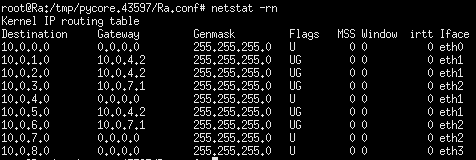
\includegraphics[width=12cm]{12.png}\par\caption{\textit{Fig. 32 - Tabela de Encaminhamento do Router A}}
\end{center}
\begin{center}
    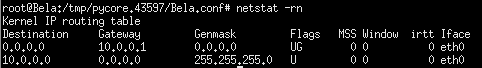
\includegraphics[width = 12cm]{123.png}\par\caption{\textit{Fig. 33 - Tabela de encaminhamento do portátil Bela}}
\end{center}

\hspace{0.5cm}No que diz respeito à figura 32 (Tabela de encaminhamento do Router A) temos que para
qualquer rede de destino existe um \textit{Gateway} para onde o tráfego deve ser direcionado. Contudo, em algumas linhas, verifica-se que o \textit{Gateway} é \textbf{0.0.0.0.} 
Isto significa que não existe um \textit{Gateway} para aquele destino em concreto. Este facto é comprovado com a falta da \textit{flag G} na mesma linha. O que acontece nestes casos é que com a ajuda do protocolo \textbf{ARP} se encontra o endereço
\textbf{MAC} da máquina destino e assim se envia diretamente o tráfego.

\hspace{0.5cm}Quanto à figura 33 (Tabela de encaminhamento do portátil \textit{Bela}), como dá para verificar na imagem correspondente, só há 2 linhas.
Uma delas representa o encaminhamento do tráfego para fora da sua sub-rede e
a outra representa o tráfego para a rede local.\clearpage


\subsubsection{Alínea b)}
\textbf{Diga, justificando, se está a ser usado encaminhamento estático ou dinâmico (sugestão: analise que processos
estão a correr em cada sistema, por exemplo, ps -ax ou equivalente).}\vspace{0.35cm}

\begin{center}
    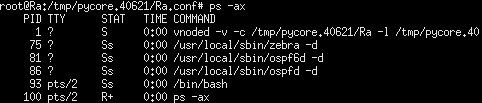
\includegraphics[width = 12cm]{22a.png}\par\caption{\textit{Fig. 34 - Execução de ps -ax no Router A}}
\end{center}
\begin{center}
    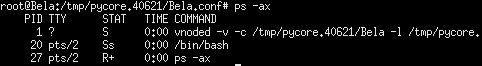
\includegraphics[width = 12cm]{22b.png}\par\caption{\textit{Fig. 35 - Execução de ps -ax no portátil Bela}}
\end{center}
\hspace{0.5cm}Ao analisar os processos em execução nas diferentes
máquinas, conclui-se que os \textit{routers} estão a usar encaminhamento dinâmico e os
portáteis e os servidores usam encaminhamento estático, como se pode concluir nas figuras 34 e 35, representadas acima.\vspace{0.35cm}


\subsubsection{Alínea c)}
\textbf{Admita que, por questões administrativas, a rota por defeito (0.0.0.0 ou default) deve ser retirada definitivamente
da tabela de encaminhamento do servidor SA. Use o comando route delete para o efeito. Que implicações tem
esta medida para os utilizadores da LEI-RC que acedem ao servidor. Justifique.}
\begin{center}
    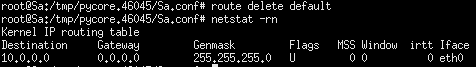
\includegraphics[width = 12cm]{23.png}\par\caption{\textit{Fig. 36}}
\end{center}
\hspace{0.5cm}A rota \textit{default} era a única que o Servidor Sa conhecia para comunicar com redes fora a sua, resultando este comando num impedimento de transmissão de informação para fora da sua rede (Rede A). Isto significa que apenas os portáteis e o \textit{router} presentes na Rede A conseguem comunicar com o Servidor Sa.
Segue-se uma tentativa de acesso de um portátil da Rede C (\textit{Ariel}) ao servidor Sa:
\begin{center}
    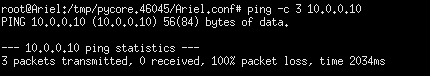
\includegraphics[width = 12cm]{232.png}\par\caption{\textit{Fig. 37}}
\end{center}
\hspace{0.5cm}Como podemos verificar, o portátil da Rede C não consegue comunicar com o servidor Sa.

\subsubsection{Alínea d)}
\textbf{Não volte a repor a rota por defeito. Adicione todas as rotas estáticas necessárias para restaurar a conectividade para o servidor SA, por forma a contornar a restrição imposta na alínea c). Utilize para o efeito o comando route \textit{add} e registe os comandos que usou.}
\begin{center}
    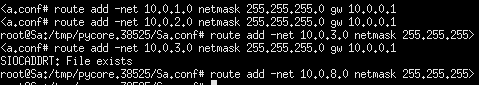
\includegraphics[width = 12cm]{24.png}\par\caption{\textit{Fig. 38}}
\end{center}
\hspace{0.5cm}Comandos utilizados:\begin{itemize}
    \item \textbf{route add -net 10.0.1.0 netmask 255.255.255.0 gw 10.0.0.1}
    \item \textbf{route add -net 10.0.2.0 netmask 255.255.255.0 gw 10.0.0.1}
    \item \textbf{route add -net 10.0.3.0 netmask 255.255.255.0 gw 10.0.0.1}
    \item \textbf{route add -net 10.0.8.0 netmask 255.255.255.0 gw 10.0.0.1}
\end{itemize}
\hspace{0.5cm}Com estes comandos adicionamos à \textit{route} os departamentos das redes B, C e D (10.0.1.0, 10.0.2.0 e 10.0.3.0 respetivamente) e o \textit{RISP} (10.0.8.0)\clearpage

\subsubsection{Alínea e)}
\textbf{Teste a nova política de encaminhamento garantindo que o servidor está novamente acessível, utilizando para o efeito o comando ping. Registe a nova tabela de encaminhamento do servidor}
\begin{center}
    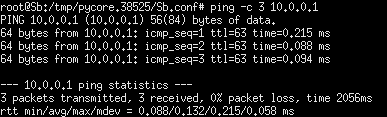
\includegraphics[width = 12cm]{25.png}\par\caption{\textit{Fig. 39 - Ping entre Servidor Sb e Servidor Sa}}
\end{center}
\begin{center}
    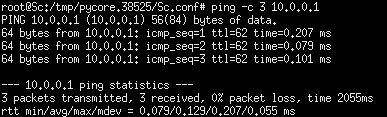
\includegraphics[width = 12cm]{252.png}\par\caption{\textit{Fig. 40 - Ping entre Servidor Sc e Servidor Sa}}
\end{center}
\begin{center}
    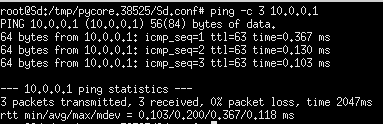
\includegraphics[width = 12cm]{253.png}\par\caption{\textit{Fig. 41 - Ping entre Servidor Sd e Servidor Sa}}
\end{center}
\begin{center}
    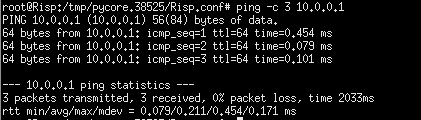
\includegraphics[width = 12cm]{254.png}\par\caption{\textit{Fig. 42 - Ping entre Risp e Servidor Sa}}
\end{center}


\subsection{Exercício 3}
\subsubsection{Alínea 1)}
\textbf{Considere que dispõe apenas do endereço de rede IP 192.168.XXX.128/25, em que XXX é o decimal correspondendo ao
seu número de grupo (PLXX). Defina um novo esquema de endereçamento para as redes dos departamentos (mantendo
as redes de acesso externo e backbone inalteradas), sabendo que o número de departamentos pode vir a aumentar no
curto prazo. Atribua endereços às interfaces dos vários sistemas envolvidos. Assuma que todos os endereços de subredes são usáveis. Justifique as opções tomadas no planeamento}.\vspace{0.35cm}

\hspace{0.5cm}Tendo em conta as instruções que nos foram dadas, nosso IP será dado por 192.168.10.128/25. Tendo em conta o nosso objetivo que é, neste caso, criar 4 sub-redes, devemos utilizar \textbf{3 \textit{bits}} (sendo que com 2 \textit{bits} poderiamos definir apenas 2 sub-redes), o que nos dá então a possibilidade de crirar 8 sub-redes, das quais duas deixaremos reservadas. A utilização de 3 \textit{bits} envolve também o incremento da máscara de 25 para 28.

\begin{center}
    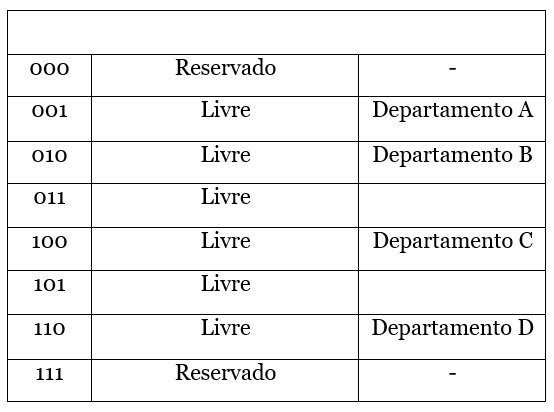
\includegraphics[width = 7cm]{3333.png}\par
\end{center}



\subsubsection{Alínea 2)}
\subsubsection{Alínea 3)}
\clearpage
\section{Conclusão}
\hspace{0.5cm}Numa primeira fase do trabalho foi-nos pedida uma análise do protocolo IPv4, para a qual utilizamos a topologia CORE de forma que nos capacitasse a análise dos datagramas e do tráfego ICMP. Isto contribuiu para um melhor entendimento do processo de transmissão de dados entre variadas máquinas ligadas à mesma rede. 

\hspace{0.5cm}Quanto à segunda parte do projeto, podemos dizer que esta se focou mais no processo de endereçamento e encaminhamento de IP. Nesta fase foi também necessário criar vários departamentos (novamente com a ajuda do CORE) de modo a averiguar a possibilidade de conexões entre si, bem como a forma como eram feitas estas conexões.

\hspace{0.5cm} No geral consideramos que este projeto foi bastante interessante e importante para adquirir mais conhecimento em relação aos conceitos abordados, bem como para pôr em prática aquilo que já sabíamos.
\cleardoublepage

\end{document}